\documentclass[10pt]{article}
\usepackage{tikz}
\usetikzlibrary{shapes.misc}
\usepackage[margin=0cm]{geometry}
\pagestyle{empty}
\tikzstyle{every node}=[cross out, draw, red]

\begin{document}

\vspace*{\fill}
\begin{center}
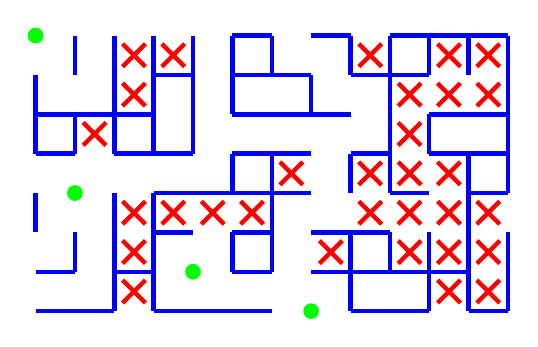
\begin{tikzpicture}[x=0.5cm, y=-0.5cm, ultra thick, blue]
% Walls
    \draw (5,0) -- (6,0);
    \draw (7,0) -- (8,0);
    \draw (9,0) -- (12,0);
    \draw (3,1) -- (4,1);
    \draw (5,1) -- (7,1);
    \draw (8,1) -- (10,1);
    \draw (0,2) -- (3,2);
    \draw (5,2) -- (8,2);
    \draw (10,2) -- (12,2);
    \draw (0,3) -- (1,3);
    \draw (2,3) -- (4,3);
    \draw (5,3) -- (7,3);
    \draw (8,3) -- (9,3);
    \draw (10,3) -- (12,3);
    \draw (3,4) -- (7,4);
    \draw (9,4) -- (10,4);
    \draw (11,4) -- (12,4);
    \draw (3,5) -- (4,5);
    \draw (5,5) -- (6,5);
    \draw (7,5) -- (9,5);
    \draw (0,6) -- (1,6);
    \draw (2,6) -- (3,6);
    \draw (5,6) -- (6,6);
    \draw (7,6) -- (11,6);
    \draw (0,7) -- (2,7);
    \draw (3,7) -- (6,7);
    \draw (8,7) -- (10,7);
    \draw (11,7) -- (12,7);
    \draw (0,1) -- (0,3);
    \draw (0,4) -- (0,5);
    \draw (1,0) -- (1,1);
    \draw (1,2) -- (1,3);
    \draw (1,5) -- (1,6);
    \draw (2,0) -- (2,3);
    \draw (2,4) -- (2,7);
    \draw (3,0) -- (3,3);
    \draw (3,4) -- (3,7);
    \draw (4,0) -- (4,3);
    \draw (5,0) -- (5,2);
    \draw (5,3) -- (5,4);
    \draw (5,5) -- (5,6);
    \draw (6,0) -- (6,1);
    \draw (6,3) -- (6,6);
    \draw (7,1) -- (7,2);
    \draw (8,0) -- (8,1);
    \draw (8,3) -- (8,4);
    \draw (8,5) -- (8,7);
    \draw (9,0) -- (9,4);
    \draw (9,5) -- (9,6);
    \draw (10,0) -- (10,1);
    \draw (10,2) -- (10,3);
    \draw (10,5) -- (10,7);
    \draw (11,0) -- (11,1);
    \draw (11,3) -- (11,7);
    \draw (12,0) -- (12,4);
    \draw (12,5) -- (12,7);
% Pillars
    \fill[green] (0,0) circle(0.2);
    \fill[green] (1,4) circle(0.2);
    \fill[green] (4,6) circle(0.2);
    \fill[green] (7,7) circle(0.2);
% Inner points in accessible cul-de-sacs
    \node at (2.5,0.5) {};
    \node at (3.5,0.5) {};
    \node at (8.5,0.5) {};
    \node at (10.5,0.5) {};
    \node at (11.5,0.5) {};
    \node at (2.5,1.5) {};
    \node at (9.5,1.5) {};
    \node at (10.5,1.5) {};
    \node at (11.5,1.5) {};
    \node at (1.5,2.5) {};
    \node at (9.5,2.5) {};
    \node at (6.5,3.5) {};
    \node at (8.5,3.5) {};
    \node at (9.5,3.5) {};
    \node at (10.5,3.5) {};
    \node at (2.5,4.5) {};
    \node at (3.5,4.5) {};
    \node at (4.5,4.5) {};
    \node at (5.5,4.5) {};
    \node at (8.5,4.5) {};
    \node at (9.5,4.5) {};
    \node at (10.5,4.5) {};
    \node at (11.5,4.5) {};
    \node at (2.5,5.5) {};
    \node at (7.5,5.5) {};
    \node at (9.5,5.5) {};
    \node at (10.5,5.5) {};
    \node at (11.5,5.5) {};
    \node at (2.5,6.5) {};
    \node at (10.5,6.5) {};
    \node at (11.5,6.5) {};
% Entry-exit paths without intersections
\end{tikzpicture}
\end{center}
\vspace*{\fill}

\end{document}
